\chapter{Enhancing the GUI}

In this chapter we'll add dashboard to our app, including
\begin{itemize}
  \item a \emph{timer} for keeping track of the player's thinking time
  \item an indicator for \emph{material evaluation}
  \item the display of \emph{captured pieces} for each player
  \item a \emph{move indicator} for the last move
  \item a display for the complete \emph{moves history}, and
  \item an \emph{info field} for displaying messages from the app.
\end{itemize}

We will also store the current game to a textfile for later use, and add a splash-screen,
allowing to display the result of a game and to switch the game mode.

Furthermore, we will give a player the option to take back a move, to offer a draw,
and to resign.

Finally, we'll revisit some \emph{special moves}.

With all that in place, our app will look like so:

\begin{center}
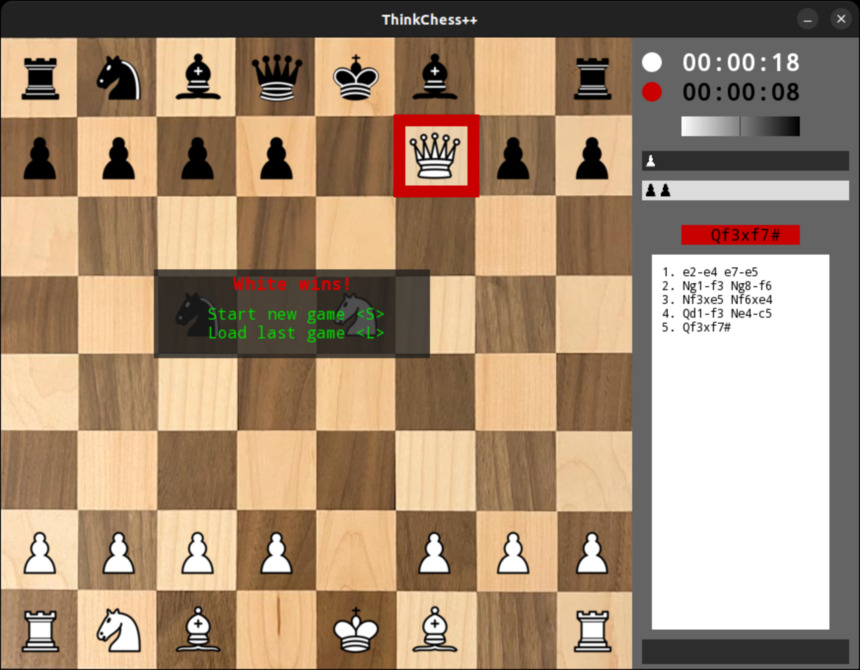
\includegraphics[width=\linewidth]{img/display.jpg}
\end{center}

\section{Refactoring}

First of all, I created a new translation unit at \texttt{app/display.cpp} and its
header file at \texttt{include/display.hpp}, which will contain all the display-oriented logic.

Next, I created another new unit at \texttt{app/position.cpp} and its header file at\\
\texttt{include/position.hpp} which contains all the move-oriented logic.\\
I moved all the functions from the old file \texttt{app/moves.cpp} to this new file and
deleted the old file.

This new file contains a new type \texttt{Position}, which holds all the position-relevant variables,
so I could delete those from the \texttt{main()} function.

\begin{cpp}
class Position {
public:
  ~Position() {}
  Position(short gs) : gamestate{gs}, player{true},
               board{8, vector<Piece*>(8)},
               mvCount{0}, castled{0}, checkmate{-1, -1},
               checked{false}, eval{0.f}
  {}

  // returns a material evaluation for both players
  pair<int, int> evaluate() {
    return evaluateBoard(board);
  }

  // take back last move
  bool takeBackMove();

  // make a move
  bool makeMove(pair<int, int> td, pair<int, int> to);

  // gamestate: 0 = game over, 1 = 2-player, 2 = analyze 
  short gamestate;

  // player on turn, starting with white
  bool player;
  
  // matrix of pieces representing the board
  vector<vector<Piece*>> board;

  // vector of moves, used as a stack
  vector<string> moves;

  // list of captured pieces, used as a stack
  vector<Piece*> captured;

  // total count of moves
  int mvCount;
  
  // castled: 0 = no, 1 = white, 2 = black, 3 = both
  short castled;
  
  // coordinates of the piece, which gave checkmate
  std::pair<int, int> checkmate;
  
  // last move gave check
  bool checked;

  // basic evaluation of positions
  float eval;

  // infotext
  string info;
};
\end{cpp}

Observe, that I've made all the member types public, in order to avoid creating all the associated
\emph{getter} and \emph{setter} functions.
This would not be a good design decision, if we were to create a library, which was intended to
be used by different clients, as those clients could harm the game logic.
But, in our case, the only client is the \texttt{main()} function of our app, and I suppose that
we know what we are doing.

With the new type \texttt{Position} in place, we can initialize all relevant variables with a single
call from inside the main function: \mintinline{cpp}{Position position(0);} and call the
\texttt{makeMove} function with just two parameters (which are the field coordinates from the board)
like so: \mintinline{cpp}{position.makeMove(touched, to)}.

Finally, I extended the viewport of the app and made it not resizable:

\begin{cpp}
auto window = sf::RenderWindow{ {870, 640u},
                                "ThinkChess++",
                                sf::Style::Close,
                                settings };

window.clear(sf::Color(100, 100, 100));
\end{cpp}

The last line just sets the background of the display area to gray (inside the game loop).

\section{Timer}

For displaying the \emph{timer}, we first have to include the \texttt{chrono} library
and define two time counters, as well as two time points:

\begin{cpp}
#include <chrono>
using namespace chrono;

unsigned wTime = 0;
unsigned bTime = 0;
steady_clock::time_point last;
last = steady_clock::now();
steady_clock::time_point now;
\end{cpp}

For calculating the current thinking time for both player, we have this code inside the
game loop, just before drawing anything:

\begin{cpp*}{linenos}
if (position.gamestate == 1) {
  now = steady_clock::now();
  if (now - last > 1s) {
    last = steady_clock::now();
    if (position.player) wTime++;
    else bTime++;
  }
}
\end{cpp*}

The code checks, wether we are in playing mode (gamestate is set to 1), and captures the current
time point (2).
If the difference between \texttt{now} and \texttt{last} is greater than one second (3), increase
the time counter for the player whose turn it is (5-6).
Remember, we have set the \texttt{sf::FramerateLimit} to 10, so this code will be called 10 times
pers second, and we cannot simply increase the time counters for each pass.

In oder to actually draw the timer, we have this code inside the game loop (directly after the
last code snippet):

\begin{cpp*}{linenos}
string timer = "";
if (position.player) {
  window.draw(wActive);
  timer = getTime(wTime);
  wTimer.setString(timer);
} else {
  window.draw(bActive);
  timer = getTime(bTime);
  bTimer.setString(timer);
}
if (position.checkmate.first != -1) {
  if (position.player) {
    bActive.setFillColor(sf::Color(200, 0, 0));
    window.draw(bActive);
  } else {
    wActive.setFillColor(sf::Color(200, 0, 0));
    window.draw(wActive);
  }
}
window.draw(wTimer);
window.draw(bTimer);
\end{cpp*}

This code also draws the indicator for the active player (the white or black circle in front of
the timer) in lines 3 and 7.
If the app has detected a checkmate (11), the active player's indicator is set to a red color (13, 16).

For that to work, we need to have the respective \texttt{sf::Sprite}s to be defined (before
entering the game loop):

\begin{cpp*}{linenos}
// set timer
sf::Text wTimer;
wTimer.setFont(noto);
wTimer.setCharacterSize(24);
wTimer.setStyle(sf::Text::Bold);
wTimer.setFillColor(sf::Color::White);
wTimer.setString("00:00:00");
wTimer.setPosition(690.f, 10.f);

sf::Text bTimer = wTimer;
bTimer.setFillColor(sf::Color::Black);
bTimer.setPosition(690.f, 40.f);

// marker for aktive player
sf::CircleShape wActive(10.f);
wActive.setPosition(650.f, 15.f);
wActive.setFillColor(sf::Color::White);

sf::CircleShape bActive(10.f);
bActive.setPosition(650.f, 45.f);
bActive.setFillColor(sf::Color::Black);
\end{cpp*}

In order to display text with SFML, we have to set a font to the \texttt{sf::Text} sprite (3),
and we also must have a font already in place (just before the last snippet):

\begin{cpp}
sf::Font noto;
if (!noto.loadFromFile("../img/NotoMono-Regular.ttf")) {
  cout << "failed to load the font\n";
  return 1;
}
\end{cpp}

I have chosen the \emph{NotoMono-Regular} font, because it is a fixed-space font and quite compact:
it only contains 897 glyphs (the images for actually drawing each character), in contrast to
more than 5,000 glyphs for fancier fonts.

The last thing missing is the function \texttt{getTime()} to convert a time counter (an unsigned
integer value) into a readable time format. This function is located inside the new
\texttt{app/display.cpp} implementation file:

\begin{cpp*}{linenos}
string getTime(unsigned t) {
  string result = "";
  unsigned h = 0;
  unsigned m = t / 60;
  unsigned s = t % 60;
  if (m >= 60) {
    h = m / 60;
    m = m % 60;
  }
  if (h < 10) {
    result.append(1, '0');
    result.append(to_string(h));
  } else {
    result.append(to_string(h));
  }
  result.append(1, ':');
  if (m < 10) {
    result.append(1, '0');
    result.append(to_string(m));
  } else {
    result.append(to_string(m));
  }
  result.append(1, ':');
  if (s < 10) {
    result.append(1, '0');
    result.append(to_string(s));
  } else {
    result.append(to_string(s));
  }
  return result;
}
\end{cpp*}

The logic is straight forward: just divide the total amount of seconds by 60 to get the minutes (4),
and take the ramainder of that calculation to get the remaining seconds (5).
If the resulting minutes are greater than 60 (6), repeat those steps to get the hours and remaining
minutes (7-8).
The rest of the code (10-29) is just for formatting: if hours, minutes, and seconds are less than 10,
insert the digit \texttt{0}  at the appropriate position.

\section{Material evaluation}

\section{Captured pieces}

\section{Move indicator}

\section{Moves history}

\section{Keyboard input}

\section{Special moves revistited}

